\subsubsection*{Rollende Kugel}

\begin{figure}[h]
	\centering
	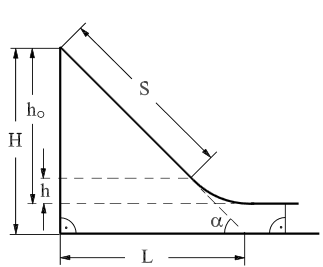
\includegraphics[width=0.7\linewidth]{res/FallrinneSkizze}
	\caption{Abbildung der Fallrinne mit den für die Auswertung relevanten Abmessungen\cite{anleitung-ws2017}.}
	\label{fig:rinneskizze}
\end{figure}


Die Kugel wurde jeweils fünfmal aus verschiedenen Höhen auf einer Fallrinne, gemäß Abbildung \ref{fig:rinneskizze}, positioniert und gegen das Pendel am Ende der Fallrinne rollen gelassen. Gemessen wurde jeweils die Auslenkung des Pendels $a$ in Abhängigkeit von $S$. Als Ablesehilfe wurde ein Reiter auf einem Messschieber genutzt welcher vor Beginn der Messung jeweils so justiert wurde, dass er etwas hinter der erwarteten Auslenkung $a$ war.
Die Auslenkung wurde anschließend gemittelt und gegen die Wurzel der Höhe aufgetragen, da die folgenden Zusammenhänge für die Näherung als vollkommen elastischen, zentralen Stoß erwartet wurden:
\begin{align}
a=\frac{2m_1}{m_1+m_2}\sqrt{\varepsilon 2 l h} \label{eq:alenkrinne}
\end{align}
Aus energetischen Betrachtungen und dem Trägheitsmoment der Kugel um die Rotationsachse folgt $\varepsilon=\frac{5}{9}$, da nur die kinetische Energie  bei dem Stoßprozess übertragen wird und die Rotationsenergie keinen Beitrag liefert.
Des weiteren gilt nach Abbildung \ref{fig:rinneskizze}:
\begin{align}
\sin \alpha &=\frac{H}{H^2+L^2}=\frac{h_0-h}{S} \\
\Rightarrow  h(S) &= h_0-\frac{S}{1+\frac{L^2}{H^2}}
\end{align}













